%
% \section{Appendix}
% 
\appendix
\section{UML Diagrams}
% A---------------------------------------------------------------
Def: Activity Diagram ~ A UML diagram that demonstrates how users interact with a given application, data flows, and branching options for workflows and processes.
% C---------------------------------------------------------------
Def: Class Diagram ~ A UML diagram that demonstrates the various classes in software, the relationships between those classes and how they depend on each other.
  \begin{figure}[h]
    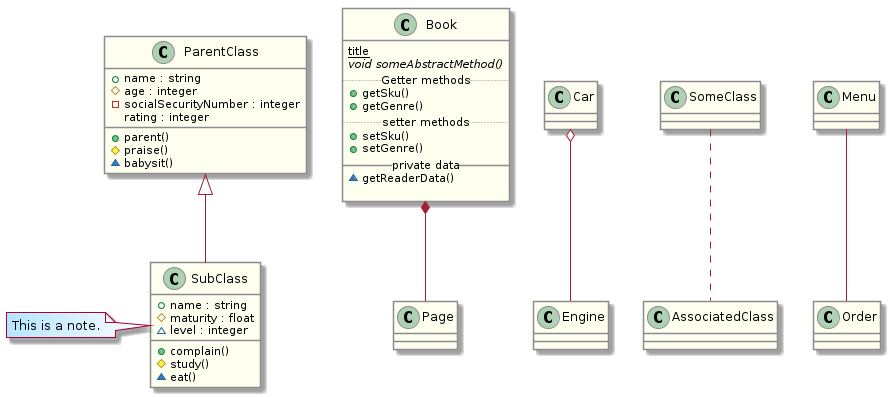
\includegraphics[width=8cm]{class-diagram-example}
  \begin{figure}
Def: Component Diagram ~ A UML diagram that demonstrates how the modular parts of software interact with each other using APIsi, interfaces or other methods. The modular parts or components include databases, web services, thin clients, thick clients, functions, libraries, and other dependencies.
% S---------------------------------------------------------------
Def: State Diagram ~ A UML diagram that describes the behavior and state of the software.
%
% eof
%
